%\title{Using the forest package to create trees in LaTeX}
% From http://tex.stackexchange.com/a/108728/23931 
\documentclass[preview,border=0]{standalone}
\usepackage[paperheight=8cm,paperwidth=6cm]{geometry}
\usepackage{graphicx}
% \usepackage{forest}
\usepackage{amsmath}
\usepackage{tikz}
\usetikzlibrary{arrows,automata,positioning}
\usepackage{bm}

\begin{document} \begin{center}
		
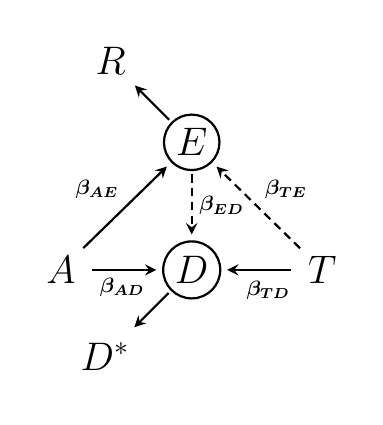
\begin{tikzpicture}[
	> = stealth, % arrow head style
	shorten > = 1pt, % don't touch arrow head to node
	auto,
	node distance = 2cm, % distance between nodes
	thick, % line style
	U/.style={circle, draw=black, inner sep=1.8pt, outer sep=1.5pt, minimum size=3mm, font=\Large},  %draw=black, fill=white
	O/.style={circle, inner sep=3.4pt, outer sep=-.75pt, minimum size=3mm, font=\Large},              %draw=white, fill=white
	]
	
	% Nodes and their relative positions
	% t = 0
    \node[O] (A) {$A$};
    \node[U] (D1) [right = .85 of A] {$D$};	
    \node[U] (E1) [above = .8 of D1] {$E$};
    \node[O] (R1) [above left = .65 of E1] {$R$};
   	\node[O] (DD1) [below left = .65 of D1] {$D^\ast$};
   	\node[O] (T) [right = .85 of D1] {$T$};
       
	% Paths connecting nodes
    \path[->] (T) edge node[outer sep=2pt, scale=.75]{$~~~\bm{\beta_{TD}}$} (D1);
    \path[->] (T) edge[densely dashed] node[above right,scale=.75]{$\bm{\beta_{TE}}$} (E1);
    \path[->] (E1) edge (R1);
    \path[->] (E1) edge[densely dashed] node[scale=.75]{$\bm{\beta_{ED}}$} (D1);
    \path[->] (A)  edge node[below,scale=.75]{$\bm{\beta_{AD}}~$} (D1);
    \path[->] (A) edge node[scale=.75]{$\bm{\beta_{AE}}$} (E1);
    \path[->] (D1) edge (DD1);
\end{tikzpicture}
	

\end{center}\end{document}
